\documentclass[11pt,a4paper]{article}

\usepackage[utf8]{inputenc}
\usepackage[T1]{fontenc}
\usepackage[margin=2cm]{geometry}
\usepackage{parskip}
\usepackage{titlesec}
\usepackage{enumitem}
\usepackage{booktabs}
\usepackage{xcolor}
\usepackage{tcolorbox}
\usepackage{graphicx}
\usepackage{hyperref}
\usepackage{fancyhdr}
\usepackage{listings}
\usepackage{fancyvrb}
\usepackage{longtable}
\usepackage{array}

\tcbuselibrary{skins,breakable}

\definecolor{accent}{RGB}{30,80,150}
\definecolor{softgray}{RGB}{245,246,248}
\definecolor{codebg}{RGB}{248,248,250}
\definecolor{warn}{RGB}{160,60,40}

\titleformat{\section}{\Large\bfseries\color{accent}}{\thesection}{0.8em}{}
\titleformat{\subsection}{\large\bfseries}{\thesubsection}{0.6em}{}

\hypersetup{colorlinks=true, linkcolor=accent, urlcolor=accent,
  pdftitle={AgentIA --- Agents, Prompts and the LangGraph},
  pdfauthor={AgentIA Engineering}}

\pagestyle{fancy}
\fancyhf{}
\fancyhead[L]{\small\color{accent}AgentIA --- Agents, Prompts and LangGraph}
\fancyhead[R]{\small\color{accent}\thepage}
\renewcommand{\headrulewidth}{0.4pt}

\lstset{
  basicstyle=\ttfamily\footnotesize, backgroundcolor=\color{codebg},
  frame=single, rulecolor=\color{softgray}, breaklines=true,
  columns=fullflexible, keepspaces=true, showstringspaces=false,
  xleftmargin=0.4em, xrightmargin=0.4em,
}

\newtcolorbox{notebox}[1][]{colback=softgray,colframe=accent,boxrule=0.4pt,
  arc=2pt,left=6pt,right=6pt,top=4pt,bottom=4pt,breakable,#1}

\title{\vspace{-1.4cm}\textbf{AgentIA --- Agents, Prompts and the LangGraph}\\[0.25cm]
\large A technical reference: every agent, its system prompt, what is prepended,
and the state machine that wires them}
\author{AgentIA Engineering}
\date{2026-09-29}

\begin{document}
\maketitle
\thispagestyle{fancy}

\begin{notebox}
\textbf{What this document is.} A verbatim technical reference for the generation
agent: the eight nodes of the LangGraph, the exact text each model-driven node is
given, what is prepended to every request, the skill, the reflector, and the state
machine that wires them together. Prompt text is loaded directly from the source
files, so it cannot drift from what the agent actually receives.
\end{notebox}

\tableofcontents
\vspace{0.4cm}

\section{The eight agents at a glance}

\begin{center}
\begin{longtable}{@{}p{0.16\textwidth}p{0.40\textwidth}p{0.34\textwidth}@{}}
\toprule
\textbf{Node} & \textbf{Role} & \textbf{Prompt} \\
\midrule
\texttt{validator} & gate the blueprint; reject a bad spec before any cost & none (deterministic) \\
\texttt{scaffolder} & build + bootstrap (pom, config, entry point) & \texttt{scaffolder.md} \\
\texttt{domain} & entities + immutable DTO records & \texttt{domain.md} \\
\texttt{service} & repository + service + implementation & \texttt{service.md} \\
\texttt{controller} & REST surface + centralized errors & \texttt{controller.md} \\
\texttt{test} & unit tests from the acceptance scenarios & \texttt{test.md} \\
\texttt{sandbox} & hermetic offline build and test & none (Docker) \\
\texttt{repair} & parse the Maven trace, apply a surgical patch & none (parser-driven) \\
\bottomrule
\end{longtable}
\end{center}

Five of the eight are model-driven; three (validator, sandbox, repair) are
deterministic and take no prompt. The five model-driven nodes share one assembly
rule, described next.

\section{What is prepended to every model request}

Every model-driven stage renders its request the same way
(\texttt{stages/runner.py}, \texttt{render\_stage\_request}). The final prompt is, in
order:

\begin{lstlisting}
[active skill prefix]               <- optional; currently EMPTY (no active.md)
<stage instruction document>        <- scaffolder.md / domain.md / ... (Section 4)

## Task payload
{ json: entities, user_stories, prior_artifacts visible to this stage }

## Output paths you own
[ "src/main/java/...", "pom.xml", ... ]

## Response format
Return ONE JSON object and nothing else -- no prose, no markdown fences.
{"artifacts": {"<workspace-relative path>": "<complete file content>"}}
\end{lstlisting}

Three properties matter. First, the \emph{skill prefix} is an optional single
document prepended before the instruction; it is currently a no-op (the active
pointer does not exist). Second, the \emph{task payload} is the stage-relevant slice
of the blueprint plus the prior artifacts, so a stage is given the entities and
contracts it may use but not the whole session. Third, the \emph{output paths} are
the stage's contractual scope from \texttt{STAGE\_ARTIFACT\_SCOPES}; the compliance
gate rejects anything outside them.

\section{The five stage prompts (verbatim)}

The five instruction documents below are the system prompts, loaded verbatim from
\texttt{backend/app/resources/instructions/}. Each must carry exactly four level-2
sections --- \emph{Technology contract}, \emph{Rules}, \emph{Output contract},
\emph{Prohibitions} --- which the loader validates before any request is sent.

\subsection{SCAFFOLDER}

\VerbatimInput[fontsize=\footnotesize,frame=single,framesep=4pt]{../backend/app/resources/instructions/scaffolder.md}

\subsection{DOMAIN}

\VerbatimInput[fontsize=\footnotesize,frame=single,framesep=4pt]{../backend/app/resources/instructions/domain.md}

\subsection{SERVICE}

\VerbatimInput[fontsize=\footnotesize,frame=single,framesep=4pt]{../backend/app/resources/instructions/service.md}

\subsection{CONTROLLER}

\VerbatimInput[fontsize=\footnotesize,frame=single,framesep=4pt]{../backend/app/resources/instructions/controller.md}

\subsection{TEST}

\VerbatimInput[fontsize=\footnotesize,frame=single,framesep=4pt]{../backend/app/resources/instructions/test.md}

\section{The skill}

A single skill document exists and is populated: \texttt{layer\_architecture.md}
(task-level; one class per layer; depend only on the layer immediately below; never
import a repository from a controller). Two further skills ---
\texttt{exception\_handling.md} and \texttt{mockito\_tests.md} --- are zero bytes, and
the active pointer \texttt{skills/active.md} is absent. Consequently the skill is
defined but \textbf{not injected}: the prefix is empty, and generation is currently
identical with or without the skill slot.

\VerbatimInput[fontsize=\footnotesize,frame=single,framesep=4pt]{../backend/app/resources/skills/layer_architecture.md}

\section{The reflector prompt}

The skill-optimisation loop (features 014--015) is built but gated; when it runs, its
reflector is this prompt, adapted from SkillOpt (arXiv:2605.23904, Appendix C.2.1). It
consumes the diagnostic channel --- the rule histogram, per-stage attribution, the
build exit code, the terminal status and the verification-fallback flag --- rather
than a binary verdict.

\VerbatimInput[fontsize=\footnotesize,frame=single,framesep=4pt]{../backend/scripts/skillopt/prompts/analyst_error.md}

\section{The LangGraph state machine}

\subsection{Topology}

The graph (\texttt{graph.py}) is a linear spine with one bounded cycle, shown in
Figure~\ref{fig:workflow}. Eight nodes, three conditional routers:

\begin{lstlisting}
START -> validator
validator -> scaffolder        (else END when status == FAILED)
scaffolder -> domain -> service -> controller -> test -> sandbox
sandbox   -> END               (build_success, or status == BLOCKED)
sandbox   -> repair            (build failed and not blocked)
repair    -> sandbox           (retry)
repair    -> END               (status == BLOCKED, max attempts)
\end{lstlisting}

\begin{figure}[htbp]
  \centering
  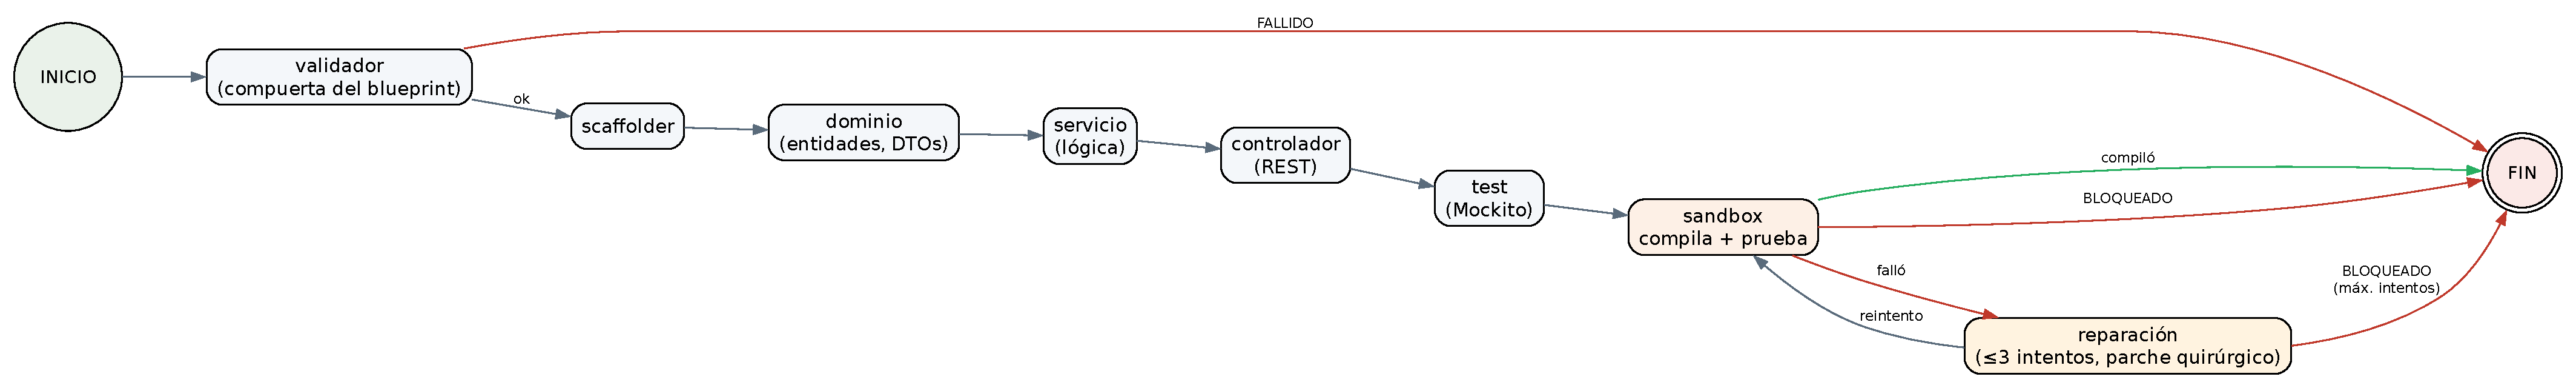
\includegraphics[width=0.92\linewidth]{fig/workflow.pdf}
  \caption{The generation state machine.}
  \label{fig:workflow}
\end{figure}

\subsection{State}

\texttt{GenerationAgentState} is a \texttt{TypedDict} with the fields tabulated below.
LangGraph filters a node's state to the declared keys, so a key that is missing from
this table is silently dropped between the entry point and the first node --- the
source of the MODEL-mode bug the \texttt{llm\_*} fields now close.

\begin{center}
\begin{longtable}{@{}p{0.34\textwidth}p{0.60\textwidth}@{}}
\toprule
\textbf{Field} & \textbf{Meaning} \\
\midrule
\texttt{session\_id, blueprint, workspace\_path} & identity, input spec, output location \\
\texttt{generated\_files} & relative path $\rightarrow$ content; the accumulated artifacts \\
\texttt{generation\_mode} & \texttt{MODEL} or \texttt{DETERMINISTIC}, decided once \\
\texttt{instruction\_set\_revision} & content digest of the instruction set in force \\
\texttt{llm\_api\_key / llm\_provider / llm\_model} & credentials for MODEL mode \\
\texttt{generation\_journal, artifact\_provenance} & per-stage outcomes and provenance \\
\texttt{repair\_attempts, max\_repair\_attempts} & the bounded-repair counter and cap \\
\texttt{build\_success, test\_metrics, verification\_fallback\_used} & the verifier's verdict \\
\texttt{last\_diagnostic} & the parsed Maven failure, for the repair node \\
\texttt{logs, status, error, current\_phase} & streaming, terminal state, phase \\
\bottomrule
\end{longtable}
\end{center}

\subsection{Mode dispatch and the entry wrapper}

\texttt{select\_generation\_mode(api\_key, provider, model)} resolves MODEL vs
DETERMINISTIC once per session: an explicit deterministic request wins; an
offline/mock selection forces deterministic; otherwise a model client is constructed
and, if it fails, the session falls back to deterministic with a recorded reason. The
compiled graph is wrapped in \texttt{\_ModeInjectingGraph}, which injects the mode at
the entry boundary via \texttt{with\_session\_generation\_mode} --- so the graph
topology, node names and edge behaviour are untouched, and a caller can always name
the mode without the seam guessing.

\end{document}
